\chapter[Создание графического интерфейса средствами Qt]{Создание графического интерфейса средствами Qt}
\section[Виджеты (Widgets)]{Виджеты (Widgets)}\label{ch13:1}
\index{Виджеты}\emph{Виджеты} (\Sys{Widgets}) --- это визуальные элементы, из которых состоит графический интерфейс
пользователя.

Примеры виджетов:

\begin{itemize}
\item Кнопка (класс \Sys{QPushButton});
\item Метка (класс \Sys{QLabel});
\item Поле ввода (класс \Sys{QLineEdit});
\item Числовое поле-счетчик (класс \Sys{QSpinBox});
\item Строка прокрутки (класс \Sys{QScrollBar}).
\end{itemize}

В \Sys{Qt} есть около 50-ти готовых классов графических элементов доступных для использования. Родительским классом для всех
виджетов является  класс \index{Класс!QWidget}\Sys{QWidget}. От него наследуются все главные свойства визуальных
элементов, которые мы тщательно рассмотрим. Исследование способов разработки программ с графическим интерфейсом начнем
с примера

\index{Создание!пустого проекта}Создадим пустой файл проекта. Запустим мастера проектов и выберем в разделе
\Sys{Projects (Проекты)} пункт \Sys{Other Project (Другой проект)}. Далее выберем тип проекта
\Sys{Empty Qt Project (Пустой проект Qt)}. К файлу проекта добавим содержимое:
\begin{lstlisting}
TEMPLATE = app
#`Модули Qt, которые мы будем использовать`
QT += widgets #`Добавляем модуль widgets для работы с виджетами (необходимо для Qt5).`
TARGET = widget #`Название исполняемого файла`
SOURCES += \
main.cpp
\end{lstlisting}

Теперь создадим простую программу с окном, в котором мы будем выводить надпись. Установим размер окна и текст его
заголовка, а также установим шрифт для \index{Класс!QLabel}надписи. Для этого создадим файл
\index{Класс!QApplication}\Sys{main.cpp} со следующим содержанием:
\begin{lstlisting}
#include <QApplication>
#include <QLabel>
int main(int lArgc, char *lArgv[])
{
//`Создаем объект QApplication, который инициализирует и настраивает оконную программу,` 
//`управляет ее выполнением с помощью цикла обработки событий`
  QApplication lApplication(lArgc, lArgv);
  QLabel lLabel;   //`Создаем виджет QLabel --- метка`
  lLabel.setText("I am Widget!");  //`Задаем текст для метки`
  lLabel.setGeometry(200, 200, 300, 150);
//`Задаем размеры --- позицию (x, y) ширину и высоту. Задаем выравнивание текста`
 lLabel.setAlignment(Qt::AlignHCenter | Qt::AlignVCenter);
//`Класс QFont используют для настройки параметров шрифта.` 
//`Выбираем семейство шрифтов Arial Black и размер 12.`
  QFont lBlackFont("Arial Black", 12);
  lLabel.setFont(lBlackFont); //`Задаем шрифт для метки`
  lLabel.show(); //`Вызываем метод show() для показа метки на экране.`
  return lApplication.exec(); //`Запускаем программу на выполнение exec() выполняет` 
//`цикл обработки событий. Программа ожидает действия пользователя и выполняет их обработку.`
}
\end{lstlisting}

\index{Класс!QFont}Как видим, элементы, из которых состоят интерфейсы в \Sys{Qt}, имеют собственные \index{Позиция и размер
виджета}\emph{позицию и размер} --- так называемую <<\emph{геометрию}>> --- и, таким образом, занимают
соответствующую прямоугольный участок на экране (см. рис.~\ref{ch13:refDrawing0}). Также каждый из элементов имеет
настройки, которые определяют его \emph{поведение и вид}.

\begin{figure}[htb]
\begin{center}
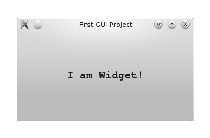
\includegraphics[width=0.3\textwidth]{img/ris_13_1}
\caption[Первый оконный проект]{Первый оконный проект}
\label{ch13:refDrawing0}
\end{center}
\end{figure}

Для создания структуры  виджеты организовывают в иерархию по принципу <<часть --- целое>>. Каждый из виджетов может
содержать другие виджеты. Такой  визуальный элемент становится <<\emph{родителем}>> (\index{Родительский
виджет}\emph{родительским виджетом}) для элементов, которые он содержит. Отметим, что такие отношения не следует
путать с наследованием в C++ --- отношениями между классами в программе. Отношения между виджетами являются отношениями
между объектами. Такие отношения порождают несколько последствий:

\begin{itemize}
\item родительский элемент будет отвечать за удаление \index{Дочерние виджеты}дочернего элемента: если родительский
виджет удалят --- то он автоматически удалит и все дочерние элементы;
\item родительский виджет размещает дочерние виджеты внутри себя, части дочерних виджетов, которые выходят  за пределы
родителя будут невидимыми;
\item часть состояния родительского виджета передается дочерним --- это касается некоторых свойств (видимость, активность)
и стилей, которые накладываются на визуальный элемент.
\end{itemize}

Виджеты, которые не имеют родителя (\index{Виджеты верхнего уровня}\emph{виджеты верхнего уровня}), имеют вид
отдельных окон в программе. Рассмотрим пример. Назовем новый проект \Sys{ParentExample}. Файл проекта будет
содержать обычные для \Sys{GUI}-проекта настройки:
\begin{lstlisting}
TEMPLATE = app
TARGET = ParentExample
QT += widgets
\end{lstlisting}

Для виджета, который мы будем использовать в качестве главного окна \index{Создание!нового класса}создадим новый класс.
Для этого в категории \Sys{Files and Classes (Файлы и классы)} выберем раздел \emph{С++} и
выберем \emph{С++ Class} (см. рис.~\ref{ch13:refDrawing1}).

\begin{figure}[htb]
\begin{center}
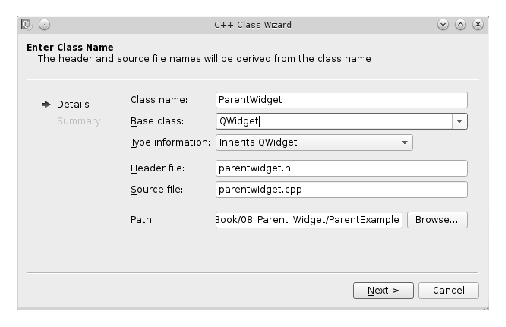
\includegraphics[width=0.7\textwidth]{img/ris_13_2}
\caption[Мастер создания нового класса]{Мастер создания нового класса}
\label{ch13:refDrawing1}
\end{center}
\end{figure}

Следующим шагом будет создание нескольких элементов на окне. Для этого откроем файл \Sys{parentwidget.cpp} и изменим
код конструктора класса. Для отображения элементов достаточно создать их в конструкторе класса и задать
\Sys{ParentWidget} как отца для них. Код \Sys{parentwidget.cpp} выглядит так:
\begin{lstlisting}
#include "parentwidget.h"
#include <QLabel>
#include <QPushButton>
#include <QLineEdit>
ParentWidget::ParentWidget(QWidget *parent) :
QWidget(parent)
{
//`Создаем метку, указывая родительский виджет --- this, то есть экземпляр класса ParentWidget.`
QLabel *lLabel=new QLabel(this);
//`Позиция относительно левого верхнего угла родительского виджета.`
lLabel->setGeometry(50, 0, 100, 30);
lLabel->setText("Text Label");       //`Текст на метке.`
//`Создаем кнопку, задаем <<родителя>>, геометрию и текст`
QPushButton *lPushButton = new QPushButton(this);
lPushButton->setGeometry(50, 50, 100, 30);
lPushButton->setText("PushButton");
//`Создаем поле ввода, задаем <<родителя>>, геометрию и текст`
QLineEdit *lLineEdit = new QLineEdit(this);
lLineEdit->setGeometry(50, 100, 100, 30);
lLineEdit->setText("LineEdit");
lLineEdit->selectAll(); //`Выделяем текст в поле ввода (просто для примера)`
//`Наконец изменяем размер родительского виджета`
setGeometry(x(), y(), 300, 150);
//`и  задаем текст заголовка окна`
setWindowTitle("Parent Widget Example");
}
\end{lstlisting}

Поскольку родительским элементом является \Sys{ParentWidget}, то метка (\Sys{QLabel}), 
кнопка (\Sys{QPushButton}) и текстовое
поле (\Sys{QLineEdit}) находятся в его пределах. Позицию дочерних виджетов 
задают относительно левого верхнего угла отца. В
этом легко убедиться изменив размеры и позицию окна нашей программы. Обратите внимание 
на то, как мы создавали элементы
пользовательского интерфейса в динамической памяти используя оператор \Sys{new}. Это гарантирует, что элементы не
будут удалены после завершения работы конструктора \Sys{ParentWidget}.

Далее добавим в проект файл \Sys{main.cpp}. Наш класс наследует от 
класса \Sys{QWidget} --- базового класса для всех
визуальных элементов пользовательского интерфейса, а следовательно будет 
обладать всеми его особенностями. Создадим
экземпляр нашего класса и вызовем метод \Sys{show()} для того, чтобы показать 
его (см. рис.~\ref{ch13:refDrawing2}).
%Главный файл программы теперь имеет вид:
%\begin{lstlisting}
%#include <QApplication>
%//`Подключаем .h файл с определением нашего класса ParentWidget`
%#include "parentwidget.h"
%int main(int lArgc, char *lArgv[])
%{
%  QApplication lApplication(lArgc, lArgv);
%  //`Создаем и показываем окно программы`
%  ParentWidget lParentWidget;
%  lParentWidget.show();
%  return lApplication.exec();
%}
%\end{lstlisting}
Для удобства работы с примером необходимо немного изменить текст программы: 
\begin{lstlisting}	 
#include <QApplication> 
//`Подключаем .h файл с определением нашего класса ParentWidget` 
#include "parentwidget.h" 
int main( int lArgc , char *lArgv [] ) 
{ 
    QApplication lApplication ( lArgc , lArgv ) ; 
    //`Создаем и показываем окно программы` 
    ParentWidget lParentWidget; 
    //`Переместить окно в точку экрана с координатами 100, 200` 
    lParentWidget.move(100, 200); 
    lParentWidget.show(); 
    return lApplication . exec () ; 
}
\end{lstlisting}


\begin{figure}[htb]
\begin{center}
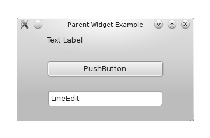
\includegraphics[width=0.3\textwidth]{img/ris_13_3}
\caption[Пример создания дочерних виджетов]{Пример создания дочерних виджетов}
\label{ch13:refDrawing2}
\end{center}
\end{figure}

\section[Компоновка (Layouts)]{Компоновка (Layouts)}
Для того, чтобы оптимально разместить виджеты на форме, необходимо учесть ряд деталей:

\begin{itemize}
\item размер соседних виджетов;
\item визуальные компоненты могут динамически изменять размер, исчезать или появляться в следствии работы логики
программы;
\item форма, в которой размещают виджеты, может динамически изменять размер при  работе программы (когда пользователь
меняет размер окна либо раскрывает его на весь экран);
\item часто нужно растянуть визуальную компоненту таким образом, чтобы она занимала все пространство формы, или же чтобы
несколько компонент занимали пространство формы пропорционально (в соответствующих пропорциях 1:1, 1:2, 3:5 и т.д.);
\item часто нужно разместить виджеты либо группы виджетов вертикально либо горизонтально на форме.
\end{itemize}

Понятно, что такая логика является довольно сложной для реализации при создании пользовательских интерфейсов разной
структуры. К счастью в арсенале Qt есть довольно мощный инструмент для упорядочивания виджетов на форме ---
\index{Компоновкщик}\emph{компоновщик}.

Компоновщик позволяет упорядочить размещение компонент, оставляя интерфейс гибким для внесения изменений, таких как
изменение размера либо количества элементов на форме. Компоновщик также может обеспечивать адекватное изменение размера
самого виджета в ответ на перемены в его наполнении.

Компоновщик не принадлежит к виджетам, не наследует от QWidget и является невидимым на форме. Он только управляет ее
размером и размещением ее содержания.

Обычно используют три основных класса компоновщика:

\begin{itemize}
\item вертикальная компоновка (класс \index{Класс!QVBoxLayout}\Sys{QVBoxLayout});
\item горизонтальная компоновка (класс \index{Класс!QHBoxLayout}\Sys{QHBoxLayout});
\item компоновка сеткой (класс \index{Класс!QGridLayout}\Sys{QGridLayout});
\end{itemize}
Для того, чтобы продемонстрировать работу с компоновками, используем предыдущий пример добавив еще несколько элементов и
сделав так, чтобы размещение элементов было пропорциональным и соответствовало изменениям размеров окна. Попытаемся
создать такой интерфейс:

\begin{itemize}
\item метки и поля ввода разместим горизонтально в одной строке;
\item создадим три такие строки с метками и полями;
\item добавим еще одну строку с двумя кнопками горизонтально и правым выравниванием.
\end{itemize}

\index{Создание!проекта с графическим интерфейсом}Создадим проект \Sys{LayoutExample}. Для этого воспользуемся
мастером новых проектов. Выберем в списке \Sys{Qt Widgets Application}. Зададим название для
проекта и настроим класс главного окна: зададим родительский класс (в выпадающем списке \Sys{Base Class} установим
\Sys{QWidget}) и снимем флажок для автоматической генерации файла формы (\Sys{Generate Form}) 
(см. рис.~\ref{ch13:refDrawing3}).

\begin{figure}[htb]
\begin{center}
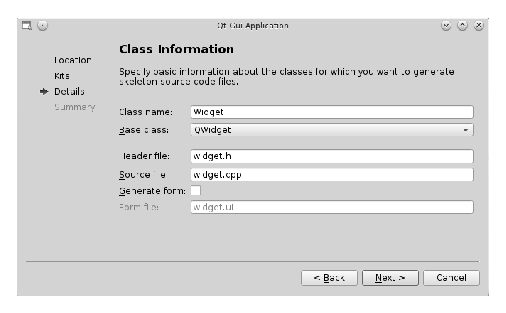
\includegraphics[width=0.7\textwidth]{img/ris_13_4}
\caption[Создание класса окна]{Создание класса окна}
\label{ch13:refDrawing3}
\end{center}
\end{figure}

Откроем файл \Sys{mainwindow.cpp} и изменим код конструктора окна:
\begin{lstlisting}
#include <QHBoxLayout>
#include <QVBoxLayout>
#include <QLabel>
#include <QLineEdit>
#include <QPushButton>
MainWindow::MainWindow(QWidget *parent) : QWidget(parent)
{
  //`Первая горизонтальная строка. Начальный текст в поле ввода`
  QLineEdit *lLineEdit = new QLineEdit("Text 1");
  //`Задаем  текст. \& --- означает комбинацию клавиш для активации виджета`
  QLabel *lLabel = new QLabel("Line Edit &1");
  //`Задаем виджет на который будет переключаться фокус ввода при нажатии Alt+1`
  lLabel->setBuddy(lLineEdit);
  //`Размещаем поле ввода и метку в одной строке`
  QHBoxLayout *lHBoxLayout = new QHBoxLayout;
  lHBoxLayout->addWidget(lLabel);
  lHBoxLayout->addWidget(lLineEdit);
  //`Вторая горизонтальная строка`
  QLineEdit *lLineEdit2 = new QLineEdit("Text 2");
  QLabel *lLabel2 = new QLabel("Line Edit &2");
  lLabel2->setBuddy(lLineEdit2);
  QHBoxLayout *lHBoxLayout2 = new QHBoxLayout;
  lHBoxLayout2->addWidget(lLabel2);
  lHBoxLayout2->addWidget(lLineEdit2);
  //`Третий ряд виджетов с кнопками`
  QPushButton *lPushButtonOk = new QPushButton("&Ok");
  QPushButton *lPushButtonCancel=new QPushButton("&Cancel");
  QHBoxLayout *lHBoxLayout3 = new QHBoxLayout;
  //`Добавим элемент-растяжку он займет все возможное свободное пространство`
  //`и "прижмет" кнопки к краю`
  lHBoxLayout3->addStretch();
  lHBoxLayout3->addWidget(lPushButtonOk);
  lHBoxLayout3->addWidget(lPushButtonCancel);
  //`Добавим компоновку вертикально в колонку`
  QVBoxLayout *lVBoxLayout = new QVBoxLayout;
  lVBoxLayout->addLayout(lHBoxLayout);
  lVBoxLayout->addLayout(lHBoxLayout2);
  lVBoxLayout->addLayout(lHBoxLayout3);
  //`Задаем компоновщик для окна`
  setLayout(lVBoxLayout);
}
\end{lstlisting}

После запуска программы получим главное окно с размещенными в компоновщиках  виджетами (см. рис.~\ref{ch13:refDrawing4}).
\begin{figure}[htb]
\begin{center}
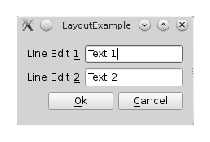
\includegraphics[width=0.3\textwidth]{img/ris_13_5}
\caption[Пример: компоновка виджетов]{Пример: компоновка виджетов}
\label{ch13:refDrawing4}
\end{center}
\end{figure}

\subsection[Компоновка сеткой (класс QGridLayout)]{Компоновка сеткой (класс QGridLayout)}

Рассмотрим работу с компоновщиками на еще одном примере. На этот раз мы создадим простую программу-калькулятор и
используем компоновщики \index{Класс!QGridLayout}\Sys{QGridLayout}.

Создадим новый проект так же, как для предыдущего примера. Добавим члены класса --- указатели на цифровые кнопки (0-9),
кнопку для сброса результата (С) и для суммирования{\textbackslash}отображения результата ($+/=$). Для создания
визуальных элементов в окне --- объявим отдельный частный метод \Sys{createWidgets()}.
\begin{lstlisting}
#include <QWidget>
//`Предварительное объявление классов`
class QPushButton;
class QLCDNumber;
class CalculatorMainWindow : public QWidget
{
  Q_OBJECT
public:
  explicit CalculatorMainWindow(QWidget *parent = 0);
  ~CalculatorMainWindow();
private:
  //`Отдельный метод для создания интерфейса программы`
  void createWidgets();
private:
  //`Цифровые кнопки`
  QPushButton *pushButton;
  QPushButton *pushButton_2;
  QPushButton *pushButton_3;
  QPushButton *pushButton_4;
  QPushButton *pushButton_5;
  QPushButton *pushButton_6;
  QPushButton *pushButton_7;
  QPushButton *pushButton_8;
  QPushButton *pushButton_9;
  QPushButton *pushButton_10;
  //`Кнопка вывода результата и суммирования`
  QPushButton *pushButtonPlus;
  //`Кнопка сброса результата`
  QPushButton *pushButtonC;
  //`Виджет --- цифровой дисплей`
  QLCDNumber *lcdNumber;
};
\end{lstlisting}


В файл реализации включим необходимые \Sys{.h}-файлы:
\begin{lstlisting}
#include <QPushButton>
#include <QGridLayout>
#include <QLCDNumber>
\end{lstlisting}

Определим метод \Sys{createWidgets()}, ответственный за создание интерфейса программы-калькулятора. В
нем создадим элемент QLCDNumber для отображения следующего слагаемого и результата. Для упрощения примера
запрограммируем только операцию сложения целых чисел. Поэтому калькулятор будет содержать только цифровые кнопки (0-9),
кнопку добавления/вывода результата и кнопку сброса результата. Все элементы пользовательского интерфейса разместим в
одной компоновке \index{Класс!QGridLayout}\Sys{QGridLayout}:
\begin{lstlisting}
void CalculatorMainWindow::createWidgets()
{
  QGridLayout *lCalcLayout = new QGridLayout;
  setLayout(lCalcLayout);
  lcdNumber = new QLCDNumber;
  pushButton = new QPushButton("1");
  pushButton_2 = new QPushButton("2");
  pushButton_3 = new QPushButton("3");
  pushButton_4 = new QPushButton("4");
  pushButton_5 = new QPushButton("5");
  pushButton_6 = new QPushButton("6");
  pushButton_7 = new QPushButton("7");
  pushButton_8 = new QPushButton("8");
  pushButton_9 = new QPushButton("9");
  pushButton_10 = new QPushButton("0");
  pushButtonC = new QPushButton("C");
  pushButtonPlus = new QPushButton("+/=");
  lCalcLayout->addWidget(lcdNumber, 0, 0 , 1, 4);
  lCalcLayout->addWidget(pushButton, 1, 0);
  lCalcLayout->addWidget(pushButton_2, 1, 1);
  lCalcLayout->addWidget(pushButton_3, 1, 2);
  lCalcLayout->addWidget(pushButton_4, 2, 0);
  lCalcLayout->addWidget(pushButton_5, 2, 1);
  lCalcLayout->addWidget(pushButton_6, 2, 2);
  lCalcLayout->addWidget(pushButton_7, 3, 0);
  lCalcLayout->addWidget(pushButton_8, 3, 1);
  lCalcLayout->addWidget(pushButton_9, 3, 2);
  lCalcLayout->addWidget(pushButton_10, 4, 0, 1, 3);
  lCalcLayout->addWidget(pushButtonC, 1, 3);
  lCalcLayout->addWidget(pushButtonPlus, 2, 3, 3, 1);
}
\end{lstlisting}

Метод \Sys{addWidget()} класса \Sys{QGridLayout} принимает в качестве параметров указатель на виджет, а также
строку и столбец для размещения виджета. Количество строк и столбцов задают заранее, оно может быть произвольным и
определяется в процессе добавления виджетов к компоновщику.
Перегруженный вариант метода \Sys{addWidget()} используем для добавления кнопок <<0>>, <<$+/=$>> и
виджета \Sys{QLCDNumber} на форму. Он принимает два дополнительных параметра. Они определяют количество ячеек по горизонтали
и по вертикали, которые будет занимать виджет в
компоновщике. Обычно каждый элемент занимает одну ячейку в
компоновщике. Последний параметр метода \Sys{addWidget()} указывает
выравнивание элемента внутри ячейки (флажки \index{Флаги!Qt::Alligment}\Sys{Qt::Alligment}).

В заключение добавим к конструктору вызов метода для создания элементов в окне.
\begin{lstlisting}
CalculatorMainWindow::CalculatorMainWindow(QWidget *parent) : QWidget(parent)
{
  resize(300, 300);
  setWindowTitle("Simple Calculator");
  createWidgets();
}
\end{lstlisting}

\section[Политики размера (Size Policies)]{Политики размера (Size Policies)}
В процессе размещения визуальные элементы и компоновки <<договариваются>> о размерах и пропорциях в окне. Компоновщики
придают размещению структурированный вид: будут ли элементы размещены в ряд (вертикально или горизонтально) либо в
сетке. В свою очередь каждый из виджетов предоставляет собственные \index{Политики размера (size
policies)}\emph{политики размера}: какое пространство будет занимать каждый визуальный элемент у ширину и высоту,
минимальный и максимальный размер для каждого из них.

Политики размера задают вызовом метода \Sys{setSizePolicy()} класса \Sys{QWidget}. Метод принимает значение для
горизонтальной и вертикальной политики изменения размера. Метод \Sys{sizeHint()} возвращает оптимальный размер
(класс \index{Класс!QSize}\Sys{QSize}), который был определен для виджета. Ниже приведены возможные значения
настройки \index{Перечисления!QSizePolicy::Policy}политик размера:

\begin{itemize}
\item \Sys{QSizePolicy::Fixed} --- \Sys{sizeHint} определяет размеры элемента. Размеры элемента  фиксированы;
\item \Sys{QSizePolicy::Minimum} --- \Sys{sizeHint}  определяет минимально возможные  размеры;
\item \Sys{QSizePolicy::Maximum} --- \Sys{sizeHint} определяет максимально возможные  размеры;
\item \Sys{QSizePolicy::Preferred} --- \Sys{sizeHint} определяет рекомендованные размеры для элемента;
\item \Sys{QSizePolicy::Expanding} --- так же как \Sys{Preferred} с тенденцией к увеличению  размера;
\item \Sys{QSizePolicy::MinimumExpanding} --- так же как \Sys{Minimum} с тенденцией к увеличению размера;
\item \Sys{QSizePolicy::Ignored} --- \Sys{sizeHint} будет игнорирован, элемент должен занимать столько места на
форме, сколько возможно.
\end{itemize}
В предыдущем примере кнопки имеют фиксированный вертикальный размер. Для того, чтобы размеры кнопок менялись как
горизонтально так и вертикально, добавим настройки политик размера метода \Sys{createWidgets()}.
\begin{lstlisting}
void CalculatorMainWindow::createWidgets()
{
	.....
//`Зададим политики размера для кнопок: горизонтальное и вертикальное изменение размера`
pushButton->setSizePolicy(QSizePolicy::Preferred,QSizePolicy::Preferred);
pushButton_2->setSizePolicy(QSizePolicy::Preferred,QSizePolicy::Preferred);
pushButton_3->setSizePolicy(QSizePolicy::Preferred,QSizePolicy::Preferred);
pushButton_4->setSizePolicy(QSizePolicy::Preferred,QSizePolicy::Preferred);
pushButton_5->setSizePolicy(QSizePolicy::Preferred,QSizePolicy::Preferred);
pushButton_6->setSizePolicy(QSizePolicy::Preferred,QSizePolicy::Preferred);
pushButton_7->setSizePolicy(QSizePolicy::Preferred,QSizePolicy::Preferred);
pushButton_8->setSizePolicy(QSizePolicy::Preferred,QSizePolicy::Preferred);
pushButton_9->setSizePolicy(QSizePolicy::Preferred,QSizePolicy::Preferred);
pushButton_10->setSizePolicy(QSizePolicy::Preferred,QSizePolicy::Preferred);
pushButtonC->setSizePolicy(QSizePolicy::Preferred,QSizePolicy::Preferred);
pushButtonPlus->setSizePolicy(QSizePolicy::Preferred,QSizePolicy::Preferred);
}
\end{lstlisting}

\index{Виджет!позиция и размер}Также размеры виджета можно жестко ограничивать с помощью методов
\Sys{setMaximumSize()} (контролирует максимальный размер элемента интерфейса) и \Sys{setMinimumSize()}
(контролирует минимальный размер). В качестве параметра они принимают объект класса \index{Класс!QSize}\Sys{QSize},
содержащий размеры элемента. Для удобства можно использовать также методы \Sys{setMinimumWidth()},
\Sys{setMinimumHeight()}, \Sys{setMaximumWidth()}, \Sys{setMaximumHeight()} для задания минимальной ширины и
высоты, а также максимальной ширины и высоты. Зададим фиксированный вертикальный размер для визуального элемента
\Sys{lcdNumber}:
\begin{lstlisting}
void CalculatorMainWindow::createWidgets()
{
  ...
  lcdNumber->setFixedHeight(50);
}
\end{lstlisting}

Результат изменения политик размера показан на рисунке~\ref{ch13:refDrawing5}.
\begin{figure}[htb]
\begin{center}
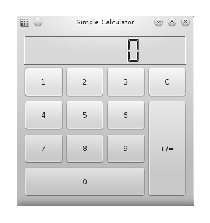
\includegraphics[width=0.3\textwidth]{img/ris_13_6}
\caption{Графический интерфейс программы-калькулятора.}
\label{ch13:refDrawing5}
\end{center}
\end{figure}

\section[Сигнально-слотовые соединения]{Сигнально-слотовые соединения}
Одной из фундаментальных возможностей в Qt является взаимодействие объектов с помощью \emph{сигнально-слотовых
соединений}. Для осознания преимуществ, которые предоставляет такая  возможность, рассмотрим как устроено
взаимодействие между объектами в программе.

Любая объектно-ориентированная программа состоит из объектов, которые взаимодействуют между собой. Каждый из объектов
обладает состоянием, которое определяет совокупность данных, которые хранит объект в данный момент. В ответ на
взаимодействие с объектом его состояние может измениться. 
Например, объект, реализующий сетевое соединение, может получить новые отправлены е
данные, а объект, реализующий кнопку на окне пользовательского интерфейса, 
может быть нажат пользователем. Таким образом объект изменил свое состояние --- 
и он может уведомить об этом другой объект посылая ему сообщение об 
изменении.
Практически это взаимодействие обычно реализуют с помощью вызова метода объекта, которому нужно
отправить сообщение. Этот метод должен выполнять соответствующие действия в ответ на изменение. Каждый объект выполняет
свою роль, а взаимодействие между ними происходит за счет взаимного вызова методов (прямого или косвенного), каждый из
которых должен выполнять собственную четкую функцию. Таким разделением получают уменьшение сложности кода --- за счет
четкого распределения ответственности между объектами --- а, следовательно, получают и гибкость, способность классов к
повторному использованию, простоту сопровождения кода. Очень важно хорошее понимание этих ключевых идей ---
разделение ответственности между объектами в программе и организации взаимодействия между ними на основе четко
определенных интерфейсов (наборов методов), вытекающих из фундаментальных понятий ООП: абстракции и инкапсуляции.

Таким образом, для реализации такого взаимодействия программисту нужно вызвать метод другого объекта в ответ на
изменение состояния. Объект, который сменил состояние, может для этого просто хранить указатель на другой объект, чей
метод нужно вызвать. В ответ на изменение состояния он будет обращаться через указатель и вызывать метод. Однако, в
таком случае теряется гибкость. Например, в случае с элементами управления в  окне программы, придется программировать
каждый элемент отдельно --- наследовать от класса элемента управления, добавлять указатель и  переопределять метод для
обработки действий пользователя с целью взаимодействия с другими объектами в программе. К тому же такая связь не может
быть динамической и задается жестко на этапе компиляции.

Конечно можно передавать указатель на метод, который будет вызываться в ответ (callback), но такой подход тоже имеет
некоторые недостатки (меньшая безопасность, всегда работает как прямой вызов метода, нужны знания о деталях
реализации). Именно поэтому в Qt используется концепция сигнально-слотовых соединений.

\index{Сигнально-слотовые соединения}\emph{Сигнально-слотовые соединения} являются простым, но в то же время важным
средством кроссплатформенного инструментария разработки \Sys{Qt}.  Один объект при изменении своего состояния может сообщить
других с помощью \index{Сигналы}\emph{сигнала}. Визуальные компоненты тоже вырабатывают сигналы в ответ на действия
пользователя (например, нажатия  кнопки, установки флага, изменения положения слайдера, редактирования текста в поле
ввода  и т.~п.). Другие объекты могут присоединиться к сигналу \index{Слоты}\emph{слотом} --- специальным методом,
который реализует некоторую функциональность  и вызывается каждый раз, когда был выпущен присоединенный к нему сигнал.
Как отмечалось ранее, сигнально-слотовые соединения могут использоваться как для взаимодействия объектов в пределах
одного потока, так и между потоками (при соответствующих условиях), также возможна организация отложенного выполнения
операций. 

Для задания соединения используют метод \Sys{connect()} класса \Sys{QObject}. Метод принимает пять параметров:

\begin{itemize}
\item указатель на объект, который посылает сигнал (sender);
\item название сигнала (signal) и его параметры, которые задаются с помощью макроса \Sys{SIGNAL()};
\item указатель на объект, который получает сигнал (receiver);
\item название слота (slot) и его параметры, которые задаются с помощью макроса \Sys{SLOT()}, или название другого
сигнала, будет эмитироваться (выпускаться) в ответ;
\item тип сигнально-слотового соединения (имеет значение по умолчанию \Sys{Qt::AutoConnection}).
\end{itemize}
В следующем примере мы продемонстрируем сигнально-слотовое соединения между кнопкой \Sys{QPushButton} и
виджетом-окном \Sys{QWidget}. В ответ на нажатие кнопки (сигнал \Sys{clicked()}), вызывается
метод-слот \Sys{close()}, который закрывает окно. Заметим, что слоты имеют спецификатор доступа
(\Sys{private/protected/public}) и вызывают их как и обычные методы класса. Этим они не отличаются от других
методов.

\lstinline!connect(lPushButton,SIGNAL(clicked()),lWindow, SLOT(close()));!

\emph{Сигнально-слотовые соединения} могут отличаться за методом вызова слота, либо за механизмом соединения.
\index{Перечисления!Qt::ConnectionType}Тип соединения можно указать при его создании:

\begin{itemize}
\item \Sys{Qt::AutoConnection} --- тип соединения по умолчанию. При соединении объектов в пределах потока ведет
себя как \Sys{Direct Connection}, иначе --- как \Sys{Queued Connection};
\item \Sys{Qt::DirectConnection} --- слот вызывается немедленно после того, как был выпущен сигнал. По сути это
напоминает обычний вызов слота как метода;
\item \Sys{Qt::QueuedConnection} --- слот выполняется, как только управления перейдет к очереди обработки
сообщений потока получателя;
\item \Sys{Qt::BlockingQueuedConnection} --- то же, что и \Sys{Queued Connection}, но поток, из которого был
выпущен сигнал блокируется, пока выполнение слота не будет завершено. Этот тип соединения должен использоваться только
когда взаимодействующие объекты находятся в разных потоках.
\item \Sys{Qt::UniqueConnection} --- этот тип соединения такой же как и \Sys{Qt::AutoConnection}, но
соединение происходит только тогда, когда оно уникально (то есть такое, которое не дублирует уже существующие
соединений).
\end{itemize}
Также с помощью соединений между слотами и сигналами может происходить передача параметров. Например, визуальный элемент
\index{Класс!QCheckBox}\Sys{QCheckBox} выпускает сигнал \Sys{toggled()} каждый раз при установке и снятии флажка.
Сигнал \Sys{toggled()} передает один параметр --- булевое значение: \Sys{true} --- если флажок установлен, 
\Sys{false} --- если нет.
Мы сможем соединить его со слотом \Sys{setChecked()} кнопки, который также принимает булевое значение и
устанавливает кнопку в положение «включено» (\Sys{true}) или «выключено» (\Sys{false}). Заметьте: мы использовали метод
\Sys{setCheckable()}, который устанавливает для кнопки режим переключения между двумя состояниями.
\begin{lstlisting}
lPushButton->setCheckable(true);
connect(lCheckBox,SIGNAL(toggled(bool)),lPushButton,SLOT(setChecked(bool)));
\end{lstlisting}

\begin{itemize}
\item порядок и тип параметров должен совпадать у объекта, который передает сигнал, и у объекта-получателя;
\item сигнал или слот получателя может опускать некоторые или все остальные параметры, при этом порядок и тип
параметров, которые остались у получателя, должны совпадать с первыми параметрами сигнала.
\end{itemize}
Один и тот же сигнал объекта может быть подключен к нескольким различным сигналам и слотам другого объекта и наоборот.
При этом последовательность, в которой будут вызываться присоединенные сигналы и слоты будет соответствовать порядку в
котором их соединили. Также надо помнить, что одно и то же соединение может быть выполнено несколько раз подряд. В
таком случае при вызове сигнала слот сработает столько же раз, сколько раз было повторно выполнено соединение. Для того,
чтобы избежать этого, необходимо передавать тип соединения \Sys{Qt::UniqueConnection} каждый раз в случаях, когда
создание повторных соединений не требуется.

Возможность создания перекрестного сигнально-слотового соединения продемонстрирована в следующем примере:
\begin{lstlisting}
connect(lCheckBox,SIGNAL(toggled(bool)),lPushButton,SLOT(setChecked(bool)));
connect(lPushButton,SIGNAL(toggled(bool)),lCheckBox,SLOT(setChecked(bool)));
\end{lstlisting}

Здесь мы видим взаимодействие между обоими элементами управления. При установке{\textbackslash}сбросе флажка кнопка
будет устанавливаться во включенное состояние или сбрасываться и наоборот.

\section[Создание сигналов (signals) и слотов (slots)]{Создание сигналов (signals) и слотов (slots)}
Для того, чтобы объект мог принимать участие в сигнально-слотовом взаимодействии, нужно удовлетворить несколько условий.
Класс, экземпляром которого является объект, должен наследовать от класса \Sys{QObject} (в случае множественного
наследования \Sys{QObject} должен быть первым в списке классов). 

Также нужно добавить к описанию класса (перед описанием любых других членов класса в секции \Sys{private}) макрос
\Sys{Q\_OBJECT}, который будет обработан метаобъектным компилятором \Sys{moc} (программа, которая выполняет
предварительную обработку текста программы при запуске \Sys{qmake} и генерирует дополнительный код для реализации
возможностей, которые предоставляет \Sys{Qt}). Далее в описании класса можно указать собственно сигналы и слоты.
\index{Сигналы}Сигналы описываются в разделе \Sys{signals}, а слоты ---  в разделе \Sys{slots}, где перед названием
раздела стоит спецификатор доступа (\Sys{public}, \Sys{private} либо \Sys{protected}). 

\index{Слоты}Слоты являются обычными методами класса, которые имеют реализацию и могут  принимать параметры и возвращать
значения. Спецификатор доступа касается только использования слота как обычного метода но не сигнально-слотовых
соединений (при получении сигнала слот будет вызван независимо от спецификатора). Также значения, которые возвращает
слот, игнорируются при сигнально-слотовом соединении. Сигналы, в отличие от слотов, не имеют реализации. Их реализация
обеспечивается метаобьектной системой \Sys{Qt}. Сигналы являются «защищенными» (\Sys{protected}) методами --- их можно
посылать из классов, которые наследуют от класса, содержащего сигнал. Сигнально-слотовые соединения могут происходить
как между объектами, так и внутри самого объекта, когда тот же объект является одновременно и отправителем сигнала и
получателем.

Создание собственных \index{Слоты!создание}слотов и использования их  в программе продемонстрируем на примере нашего
предыдущего проекта. Добавим секцию \Sys{private slots} и добавим описания слотов для обработки нажатия кнопки
калькулятора.
\begin{lstlisting}
private slots:
void slotClear();  //`Обработка нажатия кнопки сброса`
void slotButtonPressed(int pNum); //`Обработка цифровых кнопок`
void slotPlusEqual();//`Обработка кнопки сумирования/вывода результата`
\end{lstlisting}

Для сохранения результата и слагаемого, добавим частный член класса:
\begin{lstlisting}
private:
  int mSum; //`Результат`
  int mNextNumber; //`Следующее слагаемое`
\end{lstlisting}

Для упрощения примера, наш калькулятор будет выполнять только одну операцию --- сложение чисел от 0 до 9 с предыдущим
результатом и вывод результата при нажатии кнопки вывода результата и суммирования. Реализацию слотов добавим в файл
реализации класса \Sys{CalculatorMainWindow}.
\begin{lstlisting}
void CalculatorMainWindow::slotClear()
{
  lcdNumber->display(0);
  mSum = 0;
  mNextNumber = 0;
}
void CalculatorMainWindow::slotButtonPressed(int pNum)
{
  mNextNumber = pNum;
  lcdNumber->display(pNum);
}
void CalculatorMainWindow::slotPlusEqual()
{
  mSum += mNextNumber;
  lcdNumber->display(mSum);
  mNextNumber = 0;
}
\end{lstlisting}

Теперь выполним соединения для кнопок суммирования и сброса.
\begin{lstlisting}
connect(pushButtonC,SIGNAL(clicked()),this,SLOT(slotClear()),Qt::UniqueConnection);
connect(pushButtonPlus,SIGNAL(clicked()),this,SLOT(slotPlusEqual()),Qt::UniqueConnection);
\end{lstlisting}

Для реализации обработки цифровых кнопок можно использовать следующие подходы:

\begin{itemize}
\item отдельные слоты для каждого случая
\begin{itemize}
\item скорее всего будут содержать почти одинаковый код;
\item трудно поддерживать программный код;
\item трудно расширять возможности --- требует еще больше дополнительных слотов.
\end{itemize}
\item наследовать кнопку и добавить дополнительный сигнал к классу, который будет передавать значение 
\item дополнительный специализированный класс.
\end{itemize}

Однако возможен и другой подход --- использование класса \Sys{QSignalMapper}.
\index{Класс!QSignalMapper}\Sys{QSignalMapper} привязывает некоторое значение к каждому сигналу и позволяет избежать
чрезмерного дополнительного создания слотов или специализированных классов. По сути, он выполняет роль посредника между
объектами, которые посылают сигналы, и слотом, который принимает параметр, изменяющийся в зависимости от объекта,
который его выполнил. Добавим описание нового поля класса, содержащий указатель на \Sys{QSignalMapper}:
\begin{lstlisting}
//`Предварительное объявление классов`
class QSignalMapper;
...
private:
  QSignalMapper *mMapper;
\end{lstlisting}

В конструкторе класса создадим объект и свяжем каждую из кнопок с заданным для нее значением:
\begin{lstlisting}
#include <QSignalMapper>
...
connect(pushButton,SIGNAL(clicked()),mMapper,SLOT(map()),Qt::UniqueConnection);
connect(pushButton_2,SIGNAL(clicked()),mMapper,SLOT(map()),Qt::UniqueConnection);
connect(pushButton_3,SIGNAL(clicked()),mMapper,SLOT(map()),Qt::UniqueConnection);
connect(pushButton_4,SIGNAL(clicked()),mMapper,SLOT(map()),Qt::UniqueConnection);
connect(pushButton_5,SIGNAL(clicked()),mMapper,SLOT(map()),Qt::UniqueConnection);
connect(pushButton_6,SIGNAL(clicked()),mMapper,SLOT(map()),Qt::UniqueConnection);
connect(pushButton_7,SIGNAL(clicked()),mMapper,SLOT(map()),Qt::UniqueConnection);
connect(pushButton_8,SIGNAL(clicked()),mMapper,SLOT(map()),Qt::UniqueConnection);
connect(pushButton_9,SIGNAL(clicked()),mMapper,SLOT(map()),Qt::UniqueConnection);
connect(pushButton_10,SIGNAL(clicked()),mMapper,SLOT(map()),Qt::UniqueConnection);
\end{lstlisting}

После этого соединим \Sys{QSignalMapper} сигнально-слотовым соединением с нашим слотом для обработки
нажатий цифровых кнопок:
\begin{lstlisting}
connect(mMapper,SIGNAL(mapped(int)),this,SLOT(slotButtonPressed(int)),Qt::UniqueConnection);
\end{lstlisting}

Теперь программа-калькулятор готова к работе.

Заметим, что для создания соединения обычно используют метод \Sys{connect()}, но существует способ установить
соединение \index{Сигнально-слотовые соединения!автоматические}автоматически. Обычно такие соединения можно
использовать в случае, когда необходимо соединить элементы на форме созданной как \Sys{Ui}-файл с программным кодом,
реализующий обработку действий пользователя. Автоматическое соединение задают следующим образом:
\Sys{on\_<имя объекта>\_<имя сигнала> (параметры)}

Соединение происходит с помощью вызова статического метода \Sys{QMetaObject:: connectSlotsByName}.

Несмотря на относительную простоту этот метод не всегда является удобным (учитывая некоторую неочевидность, а также
способ именования слотов --- особенно когда это касается многократного их использования).

Подытожим наши знания о сигналах, слотах и сигнально-слотовых соединениях:

\index{Слоты}Слоты:
\begin{itemize}
\item слот реализуют как обычный метод класса;
\item определяют в одной из секций для слотов (\Sys{private slots}, \Sys{protected slots}, \Sys{public slots});
\item слот может возвращать значение, но это нельзя каким-либо образом использовать в сигнально-слотовом соединении;
\item произвольное количество сигналов может быть присоединено к одному слоту;
\item слот можно вызвать, как обычный метод класса.
\end{itemize}

\index{Сигналы}Сигналы:
\begin{itemize}
\item определяют в секции для сигналов (\Sys{signals});
\item сигналы всегда возвращают \Sys{void};
\item сигнал должен быть без реализации (реализацию для сигнала предоставляет метаобьектный компилятор \Sys{moc});
\item сигнал может быть присоединен к произвольному количеству слотов;
\item обычно эмитирование (выпускание) сигнала приводит к прямому вызову слота, но вызов может также быть косвенным
(зависит от типа соединения);
\item слоты при этом могут вызываться в произвольном порядке;
\item для посылки сигнала достаточно простого вызова (как в случае с методами), но предпочтительно использовать перед
вызовом макрос \Sys{emit} (используется для различия вызова метода и эмитирования сигнала, но фактически не
выполняет никакой специальной роли).
\end{itemize}

\section[Элементы графического интерфейса.]{Элементы графического интерфейса и их использование.
}
Все виджеты в \Sys{Qt} наследуют от класса \index{Класс!QWidget}\Sys{QWidget}. Класс \Sys{QWidget} предоставляет базовую
функциональность общую для всех виджетов. Среди свойств, которые наследуют от \Sys{QWidget}, --- свойство
\Sys{enabled}, которое позволяет разрешить или запретить взаимодействие пользователя с элементом управления (методы
\Sys{void setEnabled(bool)} и \Sys{bool isEnabled()}). Когда свойство установлено (логическое значение
\Sys{false}) --- визуальный элемент деактивирован и пользователь больше не может с ним взаимодействовать. Обычно такие
деактивированные элементы изменяют внешний вид, чтобы пользователь смог их отличить от активных. Свойство
\Sys{visible} (методы \Sys{void setVisible(bool)} и \Sys{bool isVisible()}) определяет видимый виджет
(значение \Sys{true}) или нет (значение \Sys{false}). Эти свойства влияют не только на сам визуальный элемент, но
и на дочерние элементы.

Кроме этих общих свойств, каждый виджет обладает собственными уникальными особенностями, которые позволяют создавать
удобные и практичные в использовании пользовательские интерфейсы.

Так, например, \emph{кнопки} (\Sys{Buttons}), очень часто употребляемый элемент управления. В общем поведение для кнопок
определяет абстрактный класс \index{Класс!QAbstractButton}\Sys{QAbstractButton}. Эти элементы могут находиться в включенном
или выключенном состояниях. Состояние можно определять с помощью свойства \Sys{checked} (метод \Sys{isChecked()}). Переключением
можно управлять с помощью свойства  \Sys{checkable (bool isCheckable(), setChеcked(bool))}.
 От класса  \Sys{QAbstractButton}
наследуют классы  \Sys{QCheckBox, QPushButton, QRadioButton, QtoolButton}.

\begin{description}
\item[\index{Класс!QPushButton}\Sys{QPushButton}] чаще используют соединяя его сигнал  \Sys{clicked()}, который вызывается
при нажатии кнопки, с другими слотами. 
\item[\index{Класс!QToolButton}\Sys{QToolButton}] является кнопкой для быстрого доступа к действиям или настройкам, которую обычно используют внутри панели инструментов.
\item[\index{Класс!QCheckBox}\Sys{QCheckBox}] --- элемент-флажок. Может находиться в включенном или выключенном
состоянии. Также может иметь третье промежуточное состояние, поддержку которого можно активировать с помощью метода
 \Sys{setTristate()}.
\item[\index{Класс!QRadioButton}\Sys{QRadioButton}] --- кнопка-переключатель. Как и флажок может находиться в включенном или выключенном
состоянии. Ее используют в группе с другими переключателями (см. класс  \Sys{QButtonGroup}) для обозначения нескольких
взаимоисключающих вариантов выбора, где только один переключатель включен, а все остальные выключены. 
\end{description}

К \index{Виджеты-контейнеры}\emph{виджетам-контейнерам} \Sys{(Containers)} относят  \Sys{QFrame, QGroupBox, QTabWidget,
QToolBox}. \index{Класс!QFrame}\Sys{QFrame} --- наиболее общий элемент. Это базовый класс для виджетов, которые имеют
обрамление. От него наследуют такие классы визуальных элементов как  \Sys{QLabel, QLCDNumber, QSplitter, QToolBox,
QStackedWidget, QAbstractScrollArea}. Может использоваться самостоятельно для отображения различных рамок.

\begin{description}
\item[\index{Класс!QGroupBox}\Sys{QGroupBox}] используют для выделения группы виджетов рамкой с надписью. Есть возможность задать
клавиатурную комбинацию, чтобы перевести фокус ввода на виджеты в группе. Не создает компоновку для группы виджетов
автоматически.
\item[\index{Класс!QTabWidget}\Sys{QTabWidget}] --- виджет для отображения виджетов внутри отдельных страниц. Предоставляет панель
вкладок и показывает виджет для текущей страницы внутри себя. Для работы необходимо создать виджет и добавить его как
страницу, а также задать имя страницы.
\item[\index{Класс!QToolBox}\Sys{QToolBox}] используют для создания вертикальной колонки виджетов со вкладками. Каждый виджет имеет
отдельную вкладку. Текущий видимый виджет соответствует текущей открытой вкладке. 
\end{description}

Также следует выделить виджеты-виды (\Sys{Views}), к которым относят \Sys{\EN{QListView},
\EN{QListWidget}, \EN{QTableView}, \EN{QTableWidget}, \EN{QTreeView}, \EN{QTreeWid\-get}}.
 Они добавляют возможность выводить информацию в виде
списков, таблиц и деревьев.  \Sys{QListView, QTableView, QTreeView} используют модель, 
как источник данных (см. абстрактный
класс  \Sys{QAbstractItemModel}).  \Sys{QListWidget, QTableWidget} и  \Sys{QTreeWidget} 
используют как самостоятельный виджет с данными,
данные добавляют поэлементно (см.  \Sys{QListWidgetItem, QTableWidgetItem, QTreeWidgetItem}). 

К элементам вывода информации (\Sys{Display widgets}) относят
\Sys{QLabel, QLCDNumber} и \Sys{QProgressBar}.
\index{Класс!QProgressBar}\Sys{QProgressBar} позволяет вывести текущий
прогресс в виде заполненной линии. \index{Класс!QLCDNumber}\Sys{QLCDNumber}
выводит целые и числа с плавающей запятой в стиле семисегментного дисплея.
\index{Класс!QLabel}\Sys{QLabel} используют для вывода различной текстовой
информации. Этот виджет также поддерживает разметку HTML4, которую можно использовать для оформления текста.

Наиболее многочисленная группа --- элементы ввода (\Sys{Input widgets}). 
К ним относят \Sys{QComboBox, QDateEdit, QDial, QDoubleSpinBo , QFontComboBox, QLineEdit,
QScrollBar, QSlider, QSpinBox, QTextEdit, QTimeEdit.}
\begin{description}
\item[\index{Класс!QComboBox}\Sys{QComboBox}] ---
выпадающий список, используемый для выбора элемента из списка
альтернатив. 
\item[\index{Класс!QDateTimeEdit}\Sys{QDateTimeEdit}] --- поле  ввода даты и времени.
Позволяет вводить и показывать время в заданном формате. Вид этого элемента наследуют также \Sys{QTimeEdit} и \Sys{QdateEdit}.
\item[\index{Класс!QDial}\Sys{QDial}] --- изменяет числовое значение по тому же
принципу, что и регуляторы на панели приборов. Наследует от абстрактного класса \Sys{QAbstractSlider}.
\item[\index{Класс!QLineEdit}\Sys{QLineEdit}] --- поле ввода. Дает возможность не только вводить текст, но и
проверять допустимость ввода (см. класс \Sys{QValidator}). Имеет режим для ввода пароля. Также возможно задать маску для
ввода значений.
\item[\index{Класс!QScrollBar}\Sys{QScrollBar}] --- элемент управления скроллингом.
Наследует от абстрактного класса \Sys{QAbstractSlider}. Каждому положению указателя соответствует значение в заданных
пределах. Часто используют для прокрутки содержимого других виджетов.
\item[\index{Класс!QSlider}\Sys{QSlider}] --- элемент, который использует
перетаскивания мышкой для ввода значений. Каждому положению указателя соответствует значение, в заданных пределах.
Наследует от абстрактного класса \Sys{QAbstractSlider}. 
\end{description}

\section[Задачи для самостоятельного решения]{Задачи для самостоятельного решения}
\begin{enumerate}
\item Добавьте к примеру калькулятора поддержку нескольких дополнительных арифметических действий (вычитание, умножение,
деление). 
\item Создайте проект с графическим интерфейсом. Разместите на окне в компоновщиках 5 различных виджетов. Соедините их
(по 2--3 между собой) сигнально-слотовыми соединениями, таким образом, чтобы они реагировали на изменения состояния друг
друга. (Например, чтобы \Sys{QScrollBar} реагировал на перемещение \Sys{QSlider}).
\item Создайте поле для игры в крестики-нолики.
Для этого разместите кнопки в компоновщиком \Sys{QGridLayout} сеткой 3х3. Также разместите в окне
надпись \Sys{QLabel}, которая будет показывать текст <<Player1>> или <<Player2>> в зависимости от того, ходит первый игрок
(крестики) или второй игрок (нолики). При нажатии на кнопку она должна менять текст в зависимости от игрока на символ
<<X>> или <<O>>. Используйте для этого класс \Sys{QSignalMapper}. Также добавьте кнопку <<Clear>>, которая будет очищать поле
(устанавливать в качестве текста для всех кнопок пустую строку). После каждого нажатия кнопки <<Clear>> порядок хода
меняется.
\end{enumerate}
